\section{Evaluation} \label{sec:parrot-eval}

We evaluated \parrot on a diverse set of \nprog programs. This set
includes \nrealprog real-world programs: \bdb, a widely used database
library~\cite{berkeleydb}; \openldap, a server implementing the
Lightweight Directory Access Protocol~\cite{openldap}; \redis, a fast
key-value data store server~\cite{redis}; \mplayer, a popular media
encoder, decoder, and player~\cite{mplayer}; \pbzip, a parallel
compression utility~\cite{pbzip2}; \pfscan, a parallel \v{grep}-like
utility~\cite{pfscan}; \aget, a parallel file download
utility~\cite{aget}; all \nstl parallel C++ STL algorithm
implementations~\cite{parallel-stl} which use \openmp; all \nimagick
parallel image processing utilities (which also use \openmp) in the
\imagick software suite~\cite{imagick} to create, edit, compose, or
convert bitmap images.  The set also includes all \nbenchmarks programs in
four widely used benchmark suites including \nparsec in
\parsec~\cite{parsec}, \nphoenix in
\phoenix~\cite{phoenix-benchmarks}, \nsplash in
\splashx~\cite{splashx}, and \nnpb in \npb~\cite{npb}.  The \phoenix
benchmark suite provides two implementations per algorithm, one using
regular Pthreads (marked with \v{-pthread} suffix) and the other using
a map-reduce library atop Pthreads.  We used complete software or
benchmark suites to avoid biasing our results.  The programs together
cover a good range of parallel programming models and idioms such as
threads, \openmp, data partition, fork-join, pipeline, map-reduce, and
workpile.  To the best of our knowledge, our evaluation of \parrot
represents \overeach more programs than any prior DMT or \smt
evaluation, and \overcombined more than all prior
evaluations combined.

Our evaluation machine was a 2.80 GHz dual-socket hex-core Intel Xeon
with 24 hyper-threading cores and 64 GB memory
running Linux 3.2.14.  Unless otherwise specified, we used the maximum
number of truly concurrent threads allowed by the machine and programs.  For 83
out of the \nprog programs, we used 24.  For 13 programs, we used 16
because they require the number of threads be a power of 
two. For \ferret, we used 18 because it requires
the number of threads to be 4$n$+2. For \mplayer, we used 8,
the max it takes. For the other
10 programs, we used 16 because they reach peak performance with
this thread count.  In scalability experiments, we varied the number of
threads from 4 to the max.
% This configuration is more aligned with today's
% servers than prior evaluations.

%% Our evaluation machines were a 2.80 GHz dual-socket hex-core Intel Xeon
%% machine with total 12 physical hyper-threading cores (24 cores) and 64 GB
%% memory running Linux 3.2.0, and a 48-core machine with four 1.9 GHz
%% 12-core AMD CPUs with 64GB memory running Linux 3.2.14.

%% Except in scalability experiments, we used the following configurations in
%% our experiments.  We used the maximum number of cores allowed by our
%% machine and the programs with peak performance.  For 86 out of the \nprog programs,
%% this number is 24.  For 13 programs it is 16, because they require the number of cores be a power
%% of two. For the other 9 programs, although it accepts 24 threads but its 
%% performance drops on our 24-core machine, so we used 16 threads for peak 
%% performance.  This configuration is more aligned with today's servers than
%% prior evaluation using only up to 8 cores.

%% the 13 programs that only accept 2^n threads are all the 7 phoenix-map reduce programs,
%% facesim, fluidanimate, fft, ocean_cp, ocean_ncp and radix.
%% the 9 programs with no peak performance at 24 threads are: kmeans, bodytrack, bodytrack-openmp,
%% rtview_raytrace, x264, barnes, fmm, radiosity, and volrend.

Unless otherwise specified, we used the following workloads.  For \bdb, we
used a popular benchmark \v{bench3n}~\cite{benchthreen}, which does
fine-grained, highly concurrent transactions. For both \openldap and
\redis, we used the benchmarks the developers themselves use, which come
with the code. For \mplayer, we used its utility \mencoder to transcode a
255 MB video (OSDI '12 keynote) from MP4 to AVI.  For \pbzip, we
compressed and decompressed a 145 MB binary file.  For \pfscan, we searched for
the keyword \v{return} in all 16K files in \v{/usr/include} on our
evaluation machine.  For \aget, we downloaded a 656 MB file. For all
\imagick programs, we used a 33 MB JPG.  For all \nstl
parallel STL algorithms, we used integer vectors with 4G elements.  For
\parsec, \splashx, and \phoenix, we used the largest workloads
because they are considered ``real'' by the benchmark authors.  For \npb, we
used the second largest workloads because the largest workloads are intended for
supercomputers. In workload sensitivity experiments, we used workloads of
3 or 4 different scales per program, typically with a 10$\times$ difference between
scales.  We also tried 15 different
types of workloads for \redis and 5 for \mplayer.  All workloads ran from
a few seconds to about 0.5 hour, using 100 or 10
repetitions respectively to bring the standard error below 1\%.
All overhead means are geometric.

We compiled all programs using \v{gcc -O2}.  To support
\openmp programs such as parallel STL algorithms, we used the GNU \libgomp.
When evaluating \parrot on the client program \aget and the server programs \openldap
and \redis, we ran both endpoints on the same machine to avoid network
latency.  \nprogadhocsync programs use ad hoc
synchronization~\cite{syncfinder:osdi10}, and we added a \v{sched\_yield}
to the busy-wait loops to make the programs work with \parrot.  \nprogtimeout
programs use \pthread timed operations, and we added \v{set\_base\_time}
(\S\ref{sec:parrot-timeout}) to them. We set the spin-wait of \parrot's scheduler
to $10^5$ cycles.  We used the default \compute timeout of 20 except 3,000
for \ferret.  Some \phoenix programs read large files, so
we ran them with a warm file cache to focus on measuring their computation
time. (Cold-cache results are unusable due to large
variations~\cite{Parrot:github}.)

%% While measuring performance results, we tried out best to choose the
%% largest typical workload for all programs.
%% For \bdb, we used a popular workload called  bench3n~\cite{bench3n},
%% which contains concurrent \v{put} and \v{get} requests with
%% transactions. For both \openldap and \redis, we used a concurrent \v{read}
%% and \v{write} workload from its own testsuite. For \mplayer, we used its utility \mencoder to 
%% convert the OSDI '12 keynote speech video (255MB) from MP4 to AVI.
%% For \pbzip, we compressed a 13MB binary file and then decompressed it.
%% For \pfscan, we scanned the keyword \v{return} from \v{/usr/include on} our evaluation machine. 
%% For \aget, we downloaded a 54MB tar bar file. For all \imagick
%% programs, we used a 3MB (full size) jpg picture taken by IPhone 4S.
%% For all \nstl parallel STL algorithms, we used integer vectors with up to 4G elements.
%% For \parsec, \splashx, \phoenix and \npb benchmark suites, we ran the largest
%% workload provided by the benchmark authors (they defined several
%% classes of workload for each benchmark program, and they considered the largest 
%% workload as the real workload). Each of these workloads take from a few 
%% seconds to half an hour. In order to avoid biasing our results on 
%% choosing workloads, we have also evaluated \parrot on three different workloads for each 
%% program (refer to figure XXX).

The rest of this section focuses on six questions:
\begin{enumerate}

\item[\S\ref{sec:parrot-ease-of-use}:] Is \parrot easy to use?  How many hints are
  needed to make the programs with \parrot fast?

\item[\S\ref{sec:parrot-performance}:] Is \parrot fast?  How effective are the
  hints?

\item[\S\ref{sec:parrot-comparison}:] How does it compare to prior systems?

\item[\S\ref{sec:parrot-sensitivity}:] How does its performance vary according
  to core counts and workload scales/types?

\item[\S\ref{sec:parrot-determinism}:] Is it deterministic in the absence of data races?

\item[\S\ref{sec:parrot-coverage}:] How much does it improve \dbug's coverage?

\end{enumerate}

\subsection{Ease of Use} \label{sec:parrot-ease-of-use}

Of all \nprog programs, \nprognohints have reasonable overhead with
default schedules, requiring no hints.  \nproglineuphints programs need a total of 
\nlineofcomputehints lines of \compute hints: \nproggenericlineuphints
need only 4 lines of generic \compute hints in \libgomp, and
\nprogspecificlineuphints need program-specific \computes
(Table~\ref{tab:parrot-computehints}).  These programs enjoy both determinism and
reasonable performance.  Only \nprognondethints programs 
need a total of \nlineofnondethints lines of \nondet hints to
trade some determinism for performance (Table~\ref{tab:parrot-nondethints}).
On average, each program needs only \hintsperprog lines.

In our experience, adding hints was straightforward.  It took roughly 0.5--2 hours per
program despite unfamiliarity with the programs.  We believe
the programs' developers would spend much less time adding better hints.
\parrot helped us deterministically reproduce the bottlenecks and identify
the synchronizations delayed by round-robin.  We used Intel \vtune~\cite{vtune} and
Linux \v{perf}~\cite{perf} performance counter-based tools to identify time-consuming
computations, and usually needed to align only the top two or three
computations.  For instance, \ferret uses a pipeline of six stages, all
serialized by the \parrot's default schedules.  We aligned only two of them to bring
the overhead down to a reasonable level.  Aligning more stages did not help.

%% Table~\ref{tab:computehints} shows that a total number of
%% \nlineofcomputehints \compute hints were added to \nproglineuphints
%% programs.  \nproggenericlineuphints programs only required a common
%% four-line stl\_generic hint.  Table~\ref{tab:nondethints} shows that
%% \nondet hints were added to \nprognondethints programs.  In average, each
%% program only needed \hintsperprog lines of hints.

%% For each program that require either \compute or \nondet hints, we only
%% spent roughly half hour to two hours on adding hints, although we were not
%% familiar with the implementation of most of the programs.  We used EIP and
%% the waiting time of each synchronization operation (optionally) recorded
%% by \parrot, and the Intel \vtune tool to inspect serialization caused by our
%% default scheduler.  The EIP showed where the serilization was in source
%% code, and how critical it was (a longer waiting time means more
%% critical). We used \vtune to identify the roughly amout of computation of
%% all the locations that have serialization, and we usually only needed to
%% take care of the top two or three of them on consuming CPU cycles. We
%% believe developers could do a much better job than us on both spending
%% less time on adding hints and writing more effective hints.

%% The determinisim and transparency of \compute hints brought lots of
%% benefits to us. Since the timeout of \compute hints is deterministic, we
%% could always get the same serialization bottlenecks over runs to runs.
%% And since the \compute hints do not affect the correctness of programs,
%% even we initially didn't add these hints properly, we were still able to
%% run programs and inspect results.

%% Table~\ref{tab:timeouts} shows that \nlineupfails programs had \compute
%% timeouts over all \nproglineuphints programs that requried \compute hints.
%% The reason of timeouts is that the workload of a program may not be evenly
%% divided by the number of threads, so some threads may handle more
%% computation than others.  Therefore, the \compute hints are suitable to
%% \parrot runtime rather than tranditional \pthread barrier, which may corrupt
%% program logic. Even timeout happened, these hints could still largely
%% speed up programs (Figure~\ref{fig:overhead-hints}).

%% We didn't need to add \compute hints to solve all seliazation in programs,
%% instead, we only needed to solve the top two or three performance-critical
%% ones (via \vtune), and we already got reasonable performance.  For
%% exmaple, in \ferret, the pipeline sync operations serialized all the six
%% parallel stages, but only two of them was significantly more
%% performance-critical than others, so we only needed to align these two. We
%% also tried to aligh all the six stages, but it turned out that the
%% \compute hints brought little performance gain.

\begin{table}[t]
\footnotesize
\centering
\begin{tabular}{lr}
{\bf Program} & {\bf Lines} \\
\hline

\mencoder, \vips, \swaptions, \freqmine, \facesim,                                 &   2 each  \\
\xtwosixfour, \radiosity, \radix, \kmeans, \\
\linearregrepthread, \linearregre, \\
\matrixmultpthread, \matrixmult, \\
\wordcntpthread, \stringmatchpthread, \\
\stringmatch, \histogrampthread, \histogram \\

\hline

\pbzip, \ferret,                                  &   3 each   \\
\kmeanspthread, \pcapthread, \pca, \wordcnt \\

\hline

\libgomp, \bodytrack  &   4 each  \\

\hline

\imagick (12 programs)                          &   25 total  \\

\end{tabular}
\caption{{\em Stats of \compute hints.} \nproglineuphints
  programs need \compute hints.  The hints in \libgomp benefit all \openmp
  programs including \imagick, STL, and \npb.} \label{tab:parrot-computehints}
\end{table}

\begin{table}[t]
\footnotesize
\centering
\begin{tabular}{lrl}
{\bf Program} & {\bf Lines} & {\bf Nondet Sync Var} \\
\hline

\pfscan                       &   2   &   \v{matches\_lock}   \\

\partition                &   2  &   \v{\_\_result\_lock}   \\

%% mutex array name: mutex[][].
\fluidanimate          &   6  &   \v{mutex[i][j]} \\

%% mutex array name: lock_array[].
\fmm                  &   2   &  \v{lock\_array[i]} \\

%% mutex array name: tasks[i].taskLock, i is thread id.
\cholesky             &   2   &  \v{tasks[i].taskLock} \\
\raytrace             &   2   &  \v{ridlock}   \\

%% mutex array name: tlock[].
\ua                       &   6   &  \v{tlock[i]} \\

\end{tabular}
\caption{{\em Stats of \nondet hints.} \nprognondethints programs need \nondet
  hints. The hints in \partition are generic for three STL programs
  \partition, \nthelement, and \partialsort. The last column shows the
  synchronization variables whose operations are made
  nondeterministic.} \label{tab:parrot-nondethints}
\end{table}

\subsection{Performance} \label{sec:parrot-performance}

\begin{figure}[t]
%%\centering
\includegraphics[width=0.57\textwidth]{parrot/figures/overhead.eps}
\vspace{-.20in}
\caption{{\em \parrot's performance normalized over nondeterministic
    execution.}  The patterns of the bars show the types of the hints the programs
  need: no hints, generic \computes in \libgomp, program-specific
  \computes, or \nondets.  The mean overhead is
  \meanoverhead (indicated by the horizontal line).} \label{fig:parrot-overhead}
\vspace{-.05in}
\end{figure}

Figure~\ref{fig:parrot-overhead} compares \parrot's performance to nondeterministic
execution.  Even with the maximum number of threads (16--24), the mean
overhead is small: \meanrealoverhead for real-world programs, \meanbenchoverhead for benchmark
programs, and \meanoverhead for all programs.
Only seven programs had over 100\% overhead.  The \ferret, \freqmine, and \is benchmarks
had dynamic load imbalance even with the starting points of the computations
aligned with \compute hints. \ua also had load 
imbalance even after \nondet hints are added.
\xtwosixfour is a pipeline program, and its overhead
comes from the \compute timeouts during the pipeline startup and
teardown.  \rtviewraytrace and \barnes have low-level
synchronizations in tight loops, and their overhead may be further reduced
with \nondets.  Four programs, \mencoder, \bodytrackopenmp, \facesim, and
\linearregrepthread, enjoyed big speedups, so we analyzed their 
executions with profiling tools. We found that the number of \mencoder's 
context switches due to synchronization decreased from 1.9M with
nondeterministic executions to 921 with \parrot.  The reason of the context
switch savings was that \parrot's round-robin scheduling reduced contention
and its synchronizations use a more efficient wait that combines spin- and
block-waits (\S\ref{sec:parrot-scheduler}).  \bodytrackopenmp and \facesim
enjoyed a similar benefit.  So did another 19 programs which had
10$\times$ fewer context switches with
\parrot~\cite{Parrot:github}. \linearregrepthread's stalled cycles were
reduced by 10$\times$ with \parrot, and we speculate that \parrot's scheduler
improved its affinity. (See~\cite{Parrot:github} for all results on
microarchitectural events.)

%% We analyzed the micro-architecture events from the executions of these
%% programs using profiling tools, and

%% and we analyzed their executions with profiling tools.  

%% njoyed big speedups, and we analyzed their
%% executions with profiling tools.  We found that \mencoder's context
%% switches reduced from 1.05M with nondeterministic execution to 3.3K with
%% \parrot. The reason was that \parrot's implementation of condition variable wait
%% uses \parrot's scheduler \v{wait}, which combines spin- and block-waits, saving
%% context switches (\S\ref{sec:scheduler}). \bodytrackopenmp had a similar 
%% pattern as that in \mencoder. \v{linear\_regression-pthread}'s
%% stalled cycles were reduced by 10$\times$ with
%% \parrot because \parrot's schedules improved affinity.

\begin{figure*}[tb]
%\centering
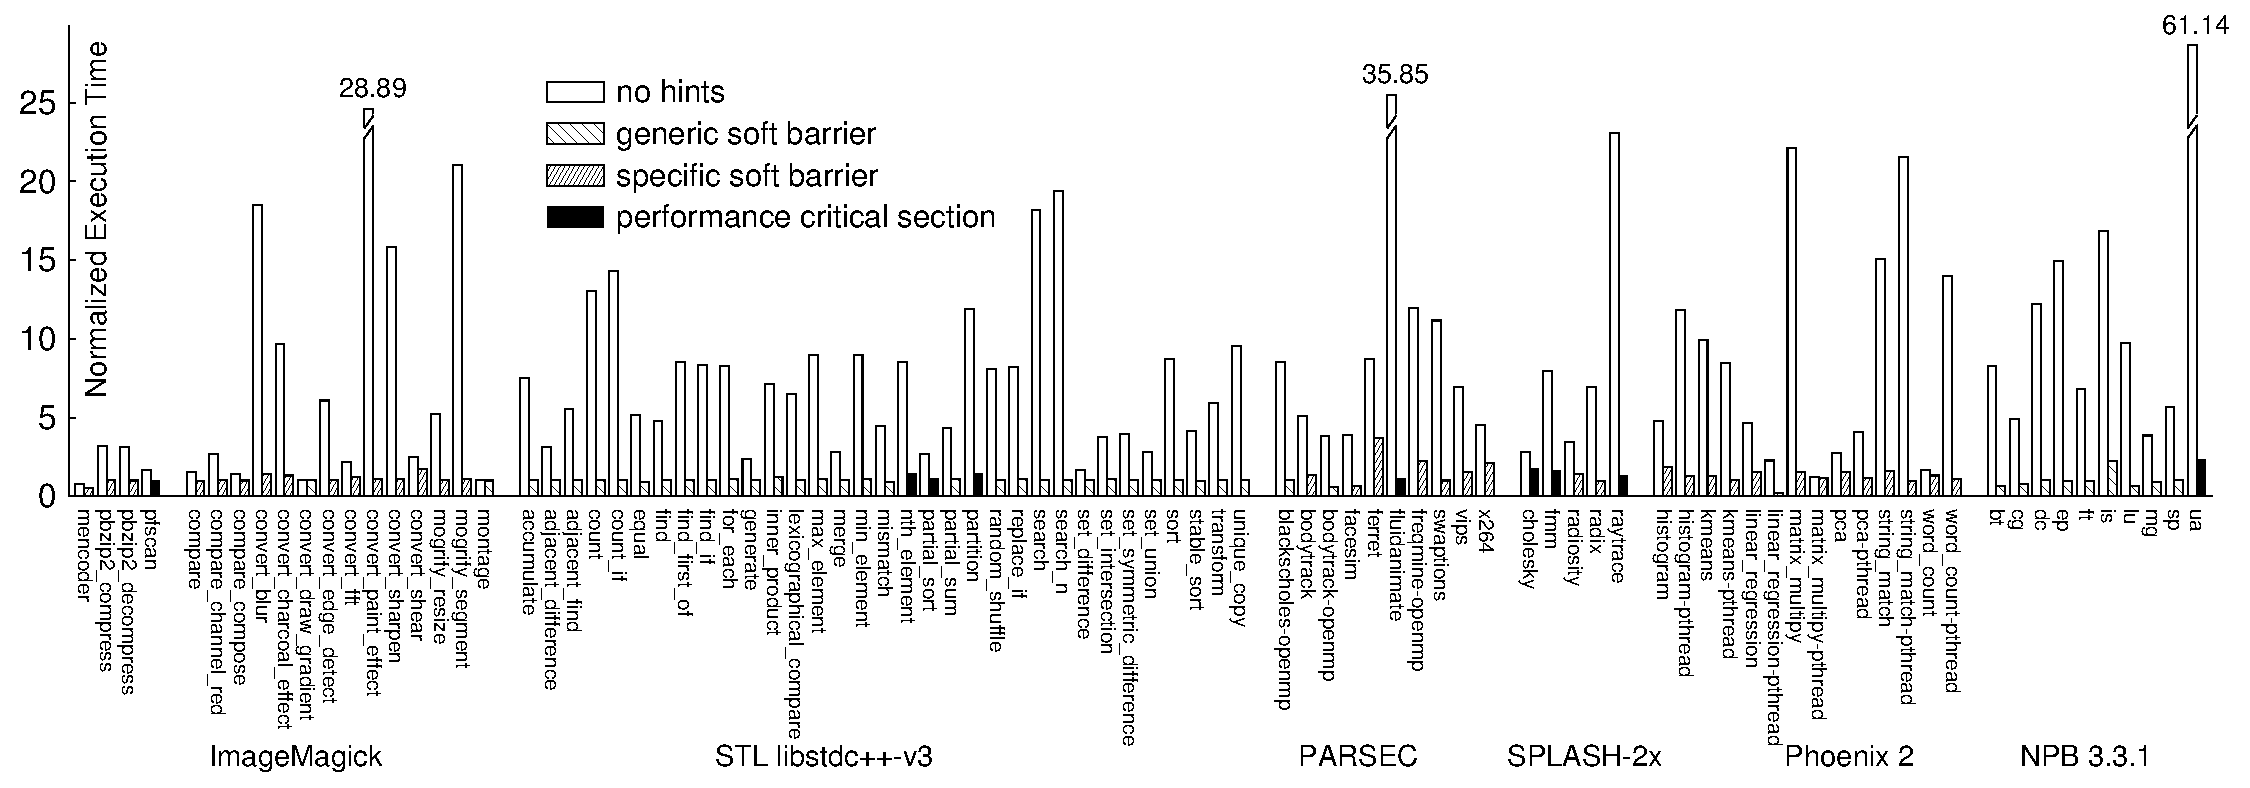
\includegraphics[width=0.57\textwidth]{parrot/figures/hints}
\vspace{-.20in}
\caption{{\em Effects of performance hints.} They reduced \parrot's overhead from \overallnohints to \overallhints.} \label{fig:parrot-overhead-hints}
\vspace{-.05in}
\end{figure*}

\begin{table}[!hb]
\footnotesize
\centering
\vspace{-.05in}
\begin{tabular}{lrr}
{\bf Program} & {\bf Success} & {\bf Timeout} \\
\hline
\convertshear                  & 725        & 1           \\
\bodytrack                        & 60,071   & 2,611     \\
\ferret                           & 699        & 2           \\
\vips                             & 3,311       & 6           \\
\xtwosixfour                             & 39,480      & 148,470      \\
\radiosity                      & 200,316     & 7,266        \\
\histogram                       & 167        & 1           \\
\kmeans                          & 1,470       & 196         \\
\pca                             & 119        & 2           \\
\pcapthread                     & 84         & 1           \\
\stringmatch                   & 64         & 1           \\
\wordcnt                     & 15,468      & 11          \\
\end{tabular}
\vspace{-.05in}
\caption{{\em \Compute successes and timeouts.}} \label{tab:parrot-timeouts}
\end{table}

Figure~\ref{fig:parrot-overhead-hints} compares \parrot's performance with and
without hints.  For all the \nprogneedhints programs that 
have hints, their mean overhead was reduced from
\overallnohints to \overallhints after hints were added. The four lines of generic
\compute hints in \libgomp (Table~\ref{tab:parrot-computehints}) 
reduced the mean overhead from \genericnolineup
to \genericlineup for \nproggenericlineuphints programs, program-specific
\computes from \specificnolineup to \specificlineup for
\nprogspecificlineuphints programs, and \nondets from \nondetnohints
to \nondethints for 9 programs.  \Computes timed out on
\nlineupfails programs (Table~\ref{tab:parrot-timeouts}), which affected neither
determinism nor correctness. The  \kmeans experienced over 10\% timeouts,
causing higher overhead. \xtwosixfour experienced many timeouts
but enjoyed partial coscheduling benefits (\S\ref{sec:parrot-hints}).

%% Table~\ref{tab:timeouts} shows that \nlineupfails programs had \compute
%% timeouts over all \nproglineuphints programs that requried \compute hints.
%% The reason of timeouts is that the workload of a program may not be evenly
%% divided by the number of threads, so some threads may handle more
%% computation than others.  Therefore, the \compute hints are suitable to
%% \parrot runtime rather than tranditional \pthread barrier, which may corrupt
%% program logic. Even timeout happened, these hints could still largely
%% speed up programs (Figure~\ref{fig:overhead-hints}).

%% generic: 6.6 times to 2.4\%, 41 programs
%% specific: 7.5 times to 33.9\%, 34 programs
%% nondet: 17.5 times to 49\%, 9 programs
%% all: 8 times to 19.6\%, 84 programs

%% First, even most of programs got 24 threads and all of them got 16+ threads, 
%% the overall overhead is still very reasonable.

%% For real applications, the overhead is negligble, and for benchmarks they are modist (recall that
%% our benchmarks are complete, and strictly run largest standard workloads, compared to other systems).

%% Second, mention the "effects of performance hints" here, ask yi-hong to provide 
%% the mean speedup XXX, which shows our hints are powerful.

%% Some programs such as mplayer and xx have significant speedup because in mplayer we saved
%% context switches (Hao provides concrete results here) and xx has better cpu affinity (by our
%% hybrid wait, yihong has studied this program).

%% Some program such as parsec mapreduce still have some siginificant amout of overhead (around 50\%)
%% because the workload is not evenly divided, so we pay some dynamic load imbalance here.

\subsection{Comparison to Prior Systems} \label{sec:parrot-comparison}

We compared \parrot's performance to \dthreads and \coredet.  We configured
both to provide the same determinism guarantee as \parrot,\footnote{While
  \kendo's determinism guarantee is closest to \parrot's, we tried and failed
  to acquire its code.}  so their overhead measured only the overhead to
make synchronizations deterministic.  One caveat is that neither system is
specially optimized for this purpose.  We managed to make only
\nprogcompared programs work with both systems because not both of them
support programming constructs such as read-write locks, semaphores,
thread local storage, network operations, and timeouts. These programs are
all benchmarks, not real-world programs.

Figure~\ref{fig:parrot-comparison} shows the comparison results.
\parrot's mean overhead is \parrotcompoverhead,
whereas \dthreads's is \dthreadssyncoverhead and \coredet's is
\coredetoverhead. 
%% When we turned on this protocol, we observed \dthreadsoverhead overhead.
\dthreads's overhead is mainly from serializing
parallel computations. \dedup, \ferret, \fluidanimate, 
\barnes, \radiosity, and \raytrace have over 500\%
overhead.  \fluidanimate is the slowest, whose threads wasted 59.3\% of their time
waiting for the other threads to do synchronizations.
%% both the internal fence (59.3\% of all threads' exeuction time) and the serialization
%% of synchronization operations (11.3\%) after the fence in \dthreads implementation.
Without \fluidanimate, \dthreads's overhead is still
\dthreadssyncoverheadnoflui.  (Performance hints may also help
\dthreads mitigate the serialization problem.)  \coredet's overhead is
mainly from counting instructions. \ferret, \fluidanimate, \barnes, and
\raytrace have over 300\% overhead.

\begin{figure}[t]
\centering
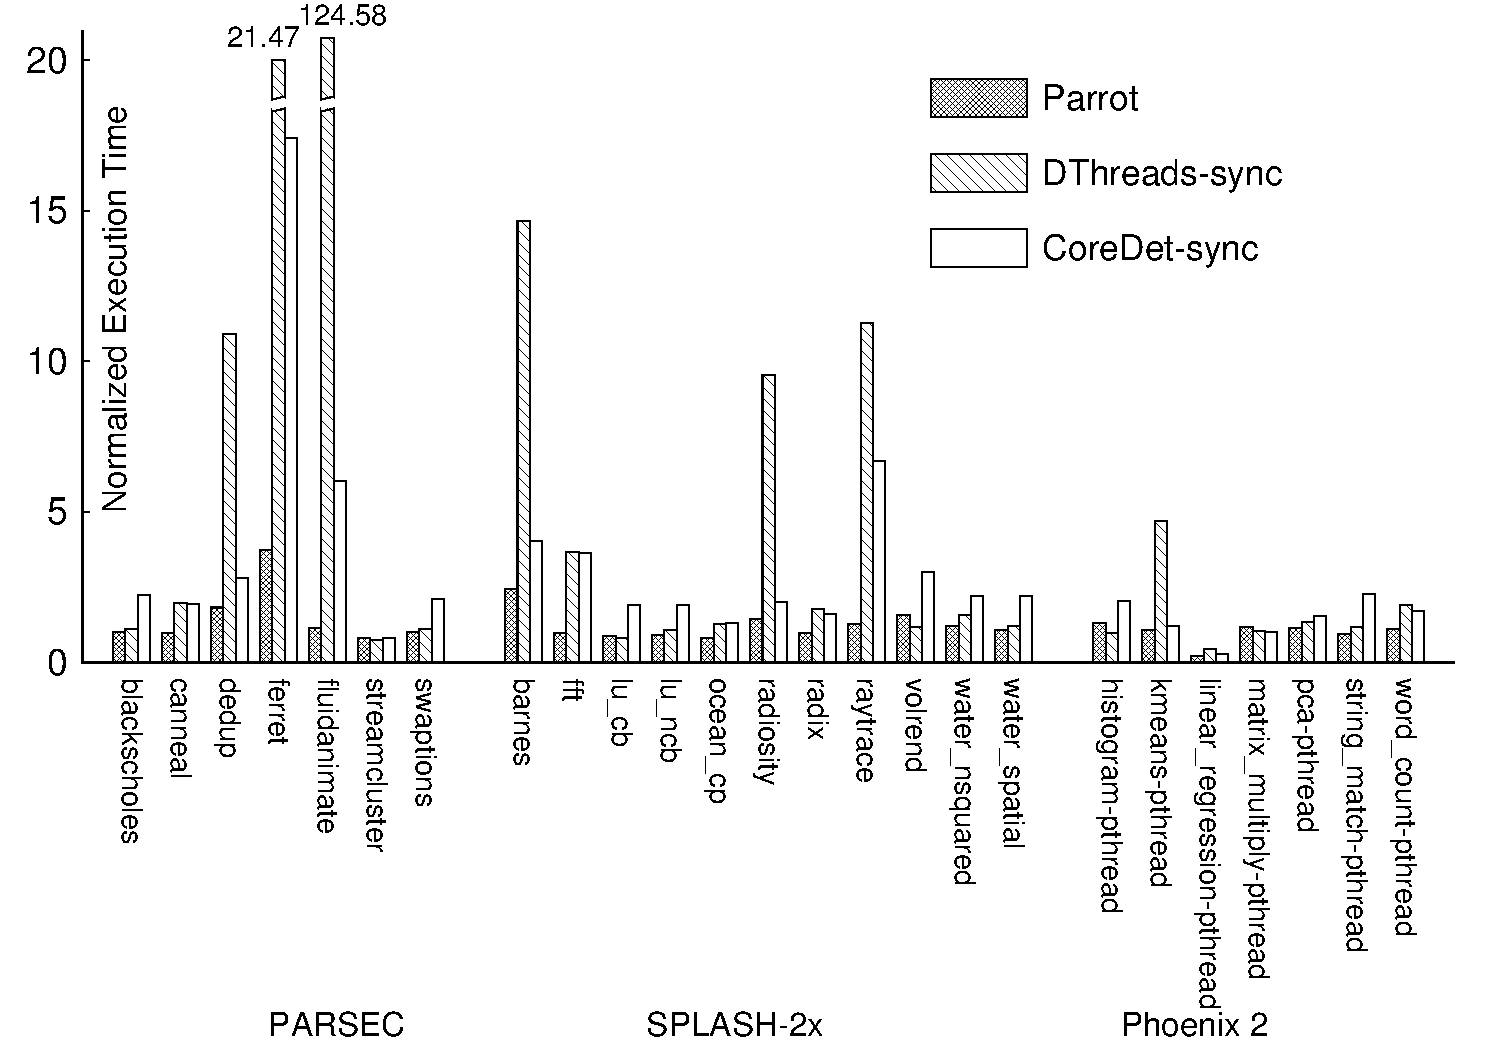
\includegraphics[width=0.57\textwidth]{parrot/figures/comparison}
\vspace{-.2in}
\caption{{\em \parrot, \dthreads, and \coredet overhead.}} \label{fig:parrot-comparison}
\vspace{-.0in}
\end{figure}

%% Note that 
%% our evaluation had more programs, (mostly) larger 
%% inputs, and more threads than the previous 
%% evaluations of the two systems. We did reduce these 
%% evaluation scales to be similar as theirs and observed 
%% compatible results as they reported.

%% First, we could run much more programs than prior systems, while the \dthreads
%% and \coredet could not run any of the real applications we have, based on the 
%% limitations (yi-hong has summarized them on a wiki page) we found.

%% Must mentioned that what modifications we changed (without affecting program 
%% logics) in those programs (such as killing shared stack objects) and made these 
%% programs work with both the other two (ask yi-hong for the modifications we made).

%% For the 30+ programs that can run with both the other two systems, we compared 
%% performance over standard largest workload and same thread settings, their 
%% overhead are \overdthreadsfull and \overcoredet times bigger than us (ask yi-hong 
%% for the mean overhead of the three systems, including ours).

%% parrot: consistently smaller
%% parrot: 79.5\%
%% dthreads: 31.9x, serialization on fluidanimate, histogram, kmeans, word\_count > 50x
%% coredet: 5.2x, string\_match-pthreads, kmeans, work\_count, string\_match > 15x

%% \begin{table}
%% \begin{tabular}{l|r}
%% {\bf System} & {\bf \# Supported} \\
%% \coredet   &  27 $\rightarrow$ 35 \\
%% \dthreads  &  24 $\rightarrow$ 31 \\
%% \parrot       & \nprog \\
%% \end{tabular}
%% \caption{{\em Number of programs supported.} The first number is the
%%   number of programs originally supported by the system, and the second
%%   after we tried our best to modify the evaluated programs to make them
%%   work with the system.}
%% \end{table}

\subsection{Scalability and Sensitivity} \label{sec:parrot-sensitivity}

%% Uncomment for the journal version of this paper

%% \begin{figure}[t]
%% \centering
%% 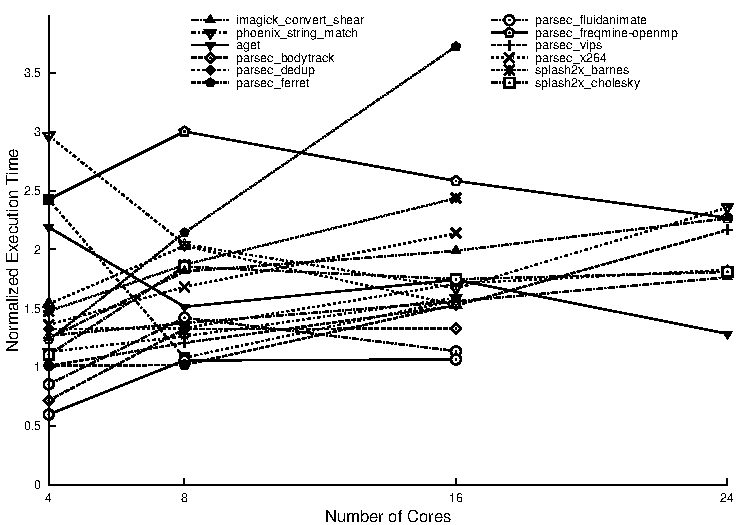
\includegraphics[width=\columnwidth]{figures/overhead_scalibility_bug}
%% \caption{{\em \parrot's scalability to the number of cores.} Legend lists
%%   only programs with over 25.0\% variance; the other programs are shown as
%%   light gray lines.} \label{fig:scalability}
%% \end{figure}

%% \begin{figure}[t]
%% \centering
%% 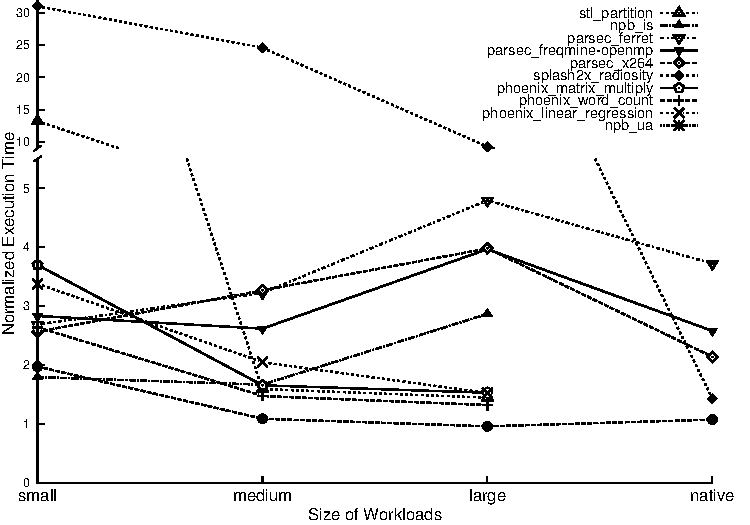
\includegraphics[width=\columnwidth]{figures/workload_sensitivity}
%% \caption{{\em \parrot's scalability to workloads.}  Legend lists only
%%   programs with over 60.0\% variance; the other programs are shown as
%%   light gray lines.} \label{fig:workloads}
%% \end{figure}
%% %% the variance is around 50%

%% Figure~\ref{fig:scalability} shows \parrot's scalability on our 24-core
%% machine. The overhead of most programs varies less than 25.0\% (light gray lines).
%% The overhead of other programs varies more, but stays below 2$\times$
%% except \ferret.  It scales worst because it uses pipeline and more threads
%% lead to more \compute timeouts during pipeline startup and teardown.

%% Figure~\ref{fig:workloads} shows \parrot's scalability on three or four
%% different scales of workloads defined by the benchmark authors.
%% The overhead of most programs varies less than 60.0\% (light gray
%% lines).  The \partition and \radiosity programs have large
%% overhead on smaller workloads because the workloads run too short.  For
%% instance, \v{radiosity}'s native workload runs for over 200s, but its
%% large workload runs for less than 3s and medium and small workloads
%% for less than 0.4s.  We also tried \redis on 15 different types of
%% workloads, and \mencoder on 5.  The results are similar to what we have
%% shown.  To summarize, the performance of \parrot and its hints are robust
%% to core counts, workload scales, and workload types.

We measured \parrot's scalability on our 24-core machine. All programs
varied within 40.0\% from each program's mean overhead across different core counts
except \ferret (57.4\%), \vips (46.7\%), \volrend (43.1\%), and
\linearregrepthread (57.1\%).  Some of these four programs use pipelines, so more
threads lead to more \compute timeouts during pipeline startup and
teardown.  We also measured \parrot's scalability on three or four different
workload scales as defined by the benchmark authors.  All programs
varied within 60\% from each program's mean overhead across different scales except
14 programs, of which 9 varied from 60\%--100\%, 3 from 100\%--150\%, and
2 above 150\%.  The 2 programs, \partition and \radiosity, went above
150\% because their smaller workloads run too short. For instance,
\v{radiosity}'s native workload runs for over 200s, but its large workload
runs for less than 3s and medium and small workloads for less than 0.4s.
We also ran \redis on 15 types of workloads, and \mencoder on
5.  The overhead did not vary much.  To summarize, \parrot's performance is
robust to core count and workload scale/type. (See~\cite{Parrot:github}
for detailed scalability results.)

%% We scaled DMT and \smt to 24 and 32 threads, a significantly high level, and 
%% we are the first DMT or \smt work to provide workload sensitivity results.
%% Each workload amout cause each program to have a execution time difference 
%% by xx times (at least 2 times, maybe? need to check). This shows our workload
%% classes are significant different.

%% Scalability over thread num, tbd (just talk about that based on the figures we 
%% have).

%% Scalability over workload, tbd. This shows our hints can tolerate workload 
%% variation pretty well (shows the quality of our hints, very important point).

%% Generally the data partition programs scale pretty well with workloads and/or 
%% thread num, because the workload are mostly balanced among threads.

%% An inteteresing point is, for all the pipeline programs we have, both workload and thread num 
%% affect overhea. We only need to use \compute hints for these programs.
%% \compute timeouts only happen at warmup and teardown of pipeline.
%% If we fix thread num and increase workload, then the overhead 
%% is smaller because steady phase could mask the overhead (Heming will add concrete results XXX).
%% If we fix workload but increase thread num, timeout would increase drastically (square).

%% redis: different workloads
%% mplayer: different conversion, different data

\subsection{Determinism} \label{sec:parrot-determinism}

We evaluated \parrot's determinism by verifying that it computed the same
schedules given the same input.  For all programs except those with
\nondets, ad hoc synchronizations, and network operations, \parrot is
deterministic.  Our current way of marking ad hoc synchronization causes
nondeterminism; annotations~\cite{syncfinder:osdi10} can solve this
problem.  We also evaluated \parrot's determinism using a modified version of
\racey~\cite{racy-stress} that protects each shared memory access with a
lock.  In \racey, each different schedule leads to a different result with
high probability.  We executed our modified \racey 1,000 times without
\parrot, and saw 1,000 different results.  With \parrot, it always computed the
same result.

%% Evaluated the determinism of sync operations with \racey. Added the same
%% mutex lock to protect each shared memory access in source code, and then
%% run both non-det (original) executions and executions with \parrot, both with
%% 1000 times. For non-det executions, each run shows different hash
%% results. For executions with xxx, each run shows same results. This shows
%% that our locks are scheduled deterministically.

\subsection{Model Checking Coverage} \label{sec:parrot-coverage}

%% We formed an \ecosys by integrating \parrot with \dbug. Within 
%% this \ecosys, \parrot determinsitically schedules all \pthread synchronizations 
%% for \dbug except those in \nondet, and \dbug systematically explores 
%% all possible schedules of network events and operations within 
%% \nondet for \parrot. But forming this \ecosys, we expect that 
%% \parrot should drastically reduce the state space of a program and
%% increase testing coverage for \dbug, and \dbug can focus on
%% exploring the schedules that matter to \parrot. We enabled 
%% dynamic partial order reduction when running both \ecosys and \dbug.
%% We focus on evaluating how well \parrot can improve 
%% testing coverage for \dbug and how effectively \dbug can explore 
%% the schedules that matter to \parrot in \ecosys.

%% because
%% checking them requires including both endpoints in the checked system
%% (\eg, to check \aget, we have to check it together with a web server). 

%% We excluded two programs \ua and \volrend, because they contain too
%% many (132M and 57M respectively) synchronization operations which
%% caused \dbug to run out of memory.

To evaluate coverage, we used small workloads and two threads per workload.
Otherwise, the time and space overhead of \dbug,
or model checking in general, becomes prohibitive. Consequently, \parrot's
reduction measured with small state spaces is a conservative estimate of
its potential.  Two programs, \volrend and \ua, were excluded because they
have too many synchronization operations (\eg, 132M for \ua), causing
\dbug to run out of memory.  Since model checking requires a closed
(no-input) system, we paired \aget with lightweight web server
\mongoose~\cite{mongoose}).  We enabled
state-of-the-art DPOR~\cite{flanagan:dynamicpo} to evaluate how much more
\parrot can reduce the state space. We checked each program for a maximum of
one day or until the checking session finished.  We then compared the
estimated state space sizes.

%% programs, and we ran both the client and server processes with \dbug and
%% \ecosys (for \aget, we setup a \mongoose server~\cite{mongoose}).


%% Three programs, \openldap, \redis, and \aget, are client or server
%% programs, and we ran both the client and server processes with \dbug and
%% \ecosys (for \aget, we setup a \mongoose server~\cite{mongoose}).

\begin{table}[!ht]
\footnotesize
\centering
\begin{tabular}{ccl}
{\bf Bin } & {\bf \# of Programs} & {\bf State Space Size with \dbug} \\
\hline
A & 27 & $1$ $\sim$ $14$ \\
B & 18 & $28$ $\sim$ $47,330$ \\
C & 25 & $3.99\times10^{6}$ $\sim$ $1.06\times10^{473}$ \\
D & 25 & $4.75\times10^{511}$ $\sim$ $2.10\times10^{19734}$ \\
%E & 1 & N/A \\
\end{tabular}
\vspace{-.05in}
\caption{{\em Estimated \dbug's state space sizes on programs with no
    \nondet nor network operation.}  } \label{tab:parrot-state-space-compute}
\vspace{-.05in}
\end{table}
% Programs are divided  into four bins based on the estimated   sizes.

%% in one day. Sorted by state space and
%%   classified by every 15. Our EcoSystem can finish testing all of them
%%   using only one deterministic schedule, and \dbug can only finish testing
%%   12 of the last 14 programs.  Seven programs of the last 14 are fork-join
%%   programs and have only one schedule.

%% Note: do not need to mention five bins, because the title of the table has mentioned this.
%% Table~\ref{tab:state-space-compute} shows all programs 
%% that need no hints or only \computes, divided into five bins based on state space size.

Table~\ref{tab:parrot-state-space-compute} bins all 95 programs that contain
(1) no network operations and (2) either no hints or only \computes. For each program,
\ecosys reduced the state space down to just one
schedule and finished in 2 seconds. \dbug alone could finish only
\nprogverifieddbug (out of 45 in bin A and B) within the time limit.
% The reduction for the bins C and D ranges from \shrinkscale.

\begin{table}[!hb]
\footnotesize
\centering
\vspace{-.05in}
\begin{tabular}{lrrr}
{\bf Program} & {\bf \dbug} & {\bf \ecosys} & {\bf Time} \\
\hline\\[-2.3ex]
%% redis smt+mc results not out yet.
%% redis                                    & $1.40\times10^{178}$    & N/A   & No       \\
\openldap                       & $2.40\times10^{2795}$        & $5.70\times10^{1048}$    & No        \\
\redis                       & $1.26\times10^{8}$        & $9.11\times10^{7}$    & No        \\
\pfscan                                   & $2.43\times10^{2117}$     & $32,268$   & $1,201$s     \\
\aget                       & $2.05\times10^{17}$        & $5.11\times10^{10}$    & No        \\
\nthelement                        & $1.35\times10^{7}$     & $8,224$   & $309$s      \\
\partialsort                       & $1.37\times10^{7}$     & $8,194$   & $307$s      \\
\partition                           & $1.37\times10^{7}$     & $8,194$   & $307$s      \\
\fluidanimate                     & $2.72\times10^{218}$        & $2.64\times10^{218}$  & No        \\
\cholesky                       & $1.81\times10^{371}$      & $5.99\times10^{152}$   & No   \\
\fmm                           & $1.25\times10^{78}$       & $2.14\times10^{54}$   & No        \\
\raytrace                       & $1.08\times10^{13863}$        &  $3.68\times10^{13755}$   & No        \\
%% UA smt+mc results not out yet.
%%\ua                                  & $>$ \v{DBL\_MAX}        & $>$ \v{DBL\_MAX}   & No        \\
\end{tabular}
\vspace{-.05in}
\caption{{\em Estimated state space sizes for programs containing
    \nondets.}  \ecosys finished 4 real-world programs (time in
  last column), and \dbug none.} \label{tab:parrot-state-space-nondet}
\end{table}

Table~\ref{tab:parrot-state-space-nondet} shows the results for all
\nprognondetandnetwork programs containing network operations or
\nondets.  For all four real-world programs \pfscan, \partition,
\nthelement, and \partialsort, \ecosys effectively explored all
schedules in seven hours or less, providing a strong reliability
guarantee.  These results also demonstrate the power of \parrot:
the programs can use the checked schedules at runtime for speed.

To summarize, \parrot reduced the state space by \shrinkscale for
\nprogshrink programs (50 programs in Table~\ref{tab:parrot-state-space-compute},
6 in Table~\ref{tab:parrot-state-space-nondet}).  It increased the number of
verified programs from \nprogverifieddbug to \nprogverifiedxxx (95
programs in Table~\ref{tab:parrot-state-space-compute}, 4 in
Table~\ref{tab:parrot-state-space-nondet}).

%  These results also demonstrate the flexibility of \parrot: once schedules
%  are checked, \parrot can use the schedules at runtime for better
%  performance.

%{\bf TODO:} Add \ua and discuss \raytrace.

%% results are promising because \parrot can safely ignore these operations in
%% \nondet and run with these programs with reasonable overhead. For the five
%% benchmark programs \fluidanimate, \cholesky, \fmm, \raytrace and \ua,
%% \ecosys could not finish exploring their state space within one day. Maybe
%% combining \ecosys with some other more effectively reduction techniques
%% could solve this problem.  Nontheless, normally people may care about
%% correctness of real applications over benchmark programs (For \redis,
%% currently we are working in progress on running it with \ecosys.).

%% Table~\ref{tab:computehints} shows all the 95 programs without 
%% \nondet hints. \ecosys can drastically reduce their huge state 
%% space to one fast (via our \compute hints) and deterministic 
%% schedule within few seconds, effectively improve testing coverage for these 
%% programs, while \dbug could only finish exploring  the schedules 
%% of 12 programs (seven of them are fork-join programs, six 
%% from phoenix, one from \parsec, and they 
%% only have one schedule) within one day run. For 81 out of 
%% the 95 programs, \ecosys proactively shrinks their state 
%% space by at least $10^{4}$, and 51 of these programs have a 
%% state space larger than $10^{10}$, so by comparing 
%% these state space with the number of schedules have been 
%% explored within one day, we estimated that the state space  
%% of these 51 programs could not be completely explored by 
%% \dbug within a few years.

%% Table~\ref{tab:nondethints} shows all the 10 programs that 
%% may contain nondeterministic events such as network or 
%% operations within \nondet. For four real applications \pfscan, 
%% \partition, \nthelement, and \partialsort, \ecosys can 
%% effectively explore all their schedules within seven hours, 
%% because \ecosys runs \parrot to deterministically schedule 
%% lots of \pthread synchronization operations and enables \dbug to 
%% focus on only exploring those schedules that matter to 
%% \parrot. We estimated that \dbug won't finish exploring 
%% scheduels for these four programs within a few years.
%% These results are promising because \parrot can 
%% safely ignore these operations in \nondet and run with 
%% these programs with reasonable overhead. For the five benchmark 
%% programs \fluidanimate, \cholesky, \fmm, \raytrace and \ua,
%% \ecosys could not finish exploring their state space within 
%% one day. Maybe combining \ecosys with some other more 
%% effectively reduction techniques could solve this problem. 
%% Nontheless, normally people may care about correctness of real applications
%% over benchmark programs (For \redis, currently we are working in progress on 
%% running it with \ecosys.).

